\documentclass[a4paper,12pt]{article}
\usepackage[utf8]{inputenc}
\usepackage[spanish]{babel}
\usepackage{graphicx}
\usepackage{color}
\begin{document}
\pagecolor[gray]{0.9}

\title {\textcolor{red}{Interpolación de Taylor}}
\author{Bolaños Florido,Cynthia. \\
Crus Guerra, Adrián.\\
Díaz Rodríguez, Diego.\\ 
\\
\\Técnicas Experimentales}
\date{15 de Mayo de 2013}
\maketitle
 \newpage
\begin{abstract}
 En este trabajo se mostrarán las características de la interpolación de {\em Taylor}, 
 además de ponerla en práctica con una función previamente dada, dando los resultados y del posible error que pueda tener.
 Además de esto también se detallará del significado de la interpolación y de las diferencias, pos y contra, 
 respecto a otras formas de interpolar. 
 Por otro lado, se hará un programa en {\tt Python}, el cual nos permitirá observar los valores de dicha interpolación de forma más breve y clara.
 \end{abstract}
  \newpage
\tableofcontents
  \newpage
 \section{\textcolor{red}{Motivación y objetivos}}
 El siguiente informe científico-técnico ha sido realizado para exponer y explicar la interpolación de una función. En particular,
 dicha interpolación se realizará mediante el método de {\em Taylor}.
 \begin{itemize}
  \item \underline{Objetivo principal:} Interpolación  de la función específica $f(x)=\frac{1}{4x}$ mediante el método de {\em Taylor}.
  \item  \underline{Objetivo específico:} Poner en práctica los conocimientos adquiridos sobre Latex y en particular con {\tt Beamer}.
 \end{itemize}
\subsection{Sección Uno}
Primero realizaremos la interpolación de la función nombrada y tras ello analizaremos el resultado.
Esto nos proporcionará la información necesaria para ver si el experimento ha sido productivo, así como la eficiencia de este.
\subsection{Sección Dos}
Una vez sacadas estas conclusiones también se tendrá en cuenta el objetivo específico mencionado anteriormente. 
Entre ellos se valorará la capacidad de:
 \begin{itemize}
  \item   Crear un archivo beamer con su correspondiente estructura.
  \item   Introducir elementos o ejemplos que aclaren el contenido teórico implementado.
  \item   Claridad, brevedad y objetividad en los contenidos expuestos.
 \end{itemize}
\newpage
\section{\textcolor{red}{Fundamentos teóricos}}
\subsection{¿Qué es la interpolación?} 
Un problema que se presenta con frecuencia en las ciencias experimentales y en ingeniería es tratar de construir una función de la que se conoce una serie de datos.
Estos datos pueden ser fruto de las observaciones realizadas en un determinado experimento en el que se relacionan dos o más variables e involucran valores de 
una función y/o de sus derivadas. El objetivo será determinar una función que verifique estos datos y que además sea fácil de construir y manipular. 
Por su sencillez y operatividad los polinomios se usan frecuentemente como funciones interpolantes.

La interpolación consiste en construir una función de la que se conoce una serie de datos que pueden ser obtenidos a partir de las observaciones realizadas en un determinado experimento.\\ 
En el caso de este trabajo la interpolación se aplica como la transformación de una función en otra, habitualmente un polinomio más sencilla para su posterior manipulación. 
\subsection{Métodos de interpolación}
Se dispone de varios métodos generales de interpolación que permiten aproximar una función por un polinomio de grado $m$. Uno de los métodos mas destacados es el de las diferencias divididas de {\em Newton}. 
Otro muy conocido es el método de la interpolación de {\em Lagrange} y por último se destaca la interpolación de {\em Hermite}, pero en este caso nosotros trabajaremos con la interpolación o serie de {\em Taylo}r. 
\subsection{Serie o interpolación de Tailor}
En matemáticas, una serie de {\em Taylor} es una representación de una función como una infinita suma de términos.
Estos términos se calculan a partir de las derivadas de la función para un determinado valor de la variable, lo que involucra un punto específico sobre la función. Si esta serie está centrada sobre el punto cero, 
se le denomina serie de {\em McLaurin}.
\newpage
\subsection{Definición}
La serie de {\em Taylor} de una función $f$ real o compleja $f(x)$ infinitamente diferenciable en el entorno de un número real o complejo a es la siguiente serie de potencias:
$$P_n(f,x,c)=f(c)+\frac{f'(c)}{1!}(x-c)+\frac{f''(c)}{2!}(x-c)^2+\cdot+\frac{f^{n)}(c)}{n!}(x-c)^n$$
Que puede ser escrito de una manera más compacta como la siguiente sumatoria:
Donde $n!$ es el factorialb de $n$ y $f(n)(a)$ denota la n-ésima derivada de $f$ para el valor $a$ de la variable respecto de la cual se deriva. La derivada de orden cero de $f$ es definida como la propia $f$ y tanto
$\left({x-a}\right)^n$ como $()!$ como $1 (()! = 1)$. En caso de ser $a= 0$, como ya se ha mencionado, la serie se denomina también de {\em Maclaurin.}
\subsection{Ventajas de la interpolación}
La interpolación de {\em Taylor} en concreto presenta tres ventajas fundamentales:
\begin{itemize}

 \item La derivación e integración de una de estas series se puede realizar término a término, que resultan operaciones triviales.
 \item Se puede utilizar para calcular valores aproximados de la función.
 \item Es posible demostrar que, si es viable la transformación de una función a una serie de{\em  Taylor}, es la óptima aproximación posible.
\end{itemize}
\newpage
\section{\textcolor{red}{Procedimiento experimental}}
A continuación expondremos los pasos que se han seguido en la elaboración del experimento desarrollado para este trabajo de investigación. 
Nos apoyaremos en gráficos y tablas que les ayudaran a reforzar y aclarar la información desarrollada.
\subsection{Descripción de los experimentos}
Para llevar a cabo la interpolación de {\em Taylor}, objetivo principal del informe, se ha empleado la sucesión de {\em Taylor}. Recodar que  la función interpolada ha sido $f(x)=\frac{1}{4x}$  y que al aplicar la sucesión de {\em Taylo}r se ha requerido obtener la derivada enésima para poder aplicar la fórmula expuesta anteriormente en los fundamentos teóricos. 

En relación a la eficiencia del proyecto, se ha analizado el resultado obtenido de la interpolación midiendo el error de este con el resultado original de la función.  
\subsection{Descripción del material}
El material utilizado ha sido el siguiente:
\begin {itemize}
\item \underline{Tipo de CPU}: 
 
 
 Pentium(R) Dual-Core CPU E5200 @ 2.50GHz 

\item \underline{Tamaño de la memoria del procesador}: 


 2048 KB

\item \underline{Vendedor GenuineIntel}:


Linux

\item \underline{Sistema operativo}:


 66-Ubuntu SMP

\item \underline{Plataforma}:


 Linuz-3.2.0-41-generic-i686-with-Ubuntu-12.04-precise

\item \underline{Version}:

2.7.3
\end{itemize}

\newpage
\subsection{Resultados obtenidos}
\begin{table}[!hbt]
\begin{center}
\begin{tabular}[c]{||l | l ||l|l||}
\hline
\hline
$x$  & $f(x)=\frac{1}{4x}$ &{\em Taylor} & Error \\
\hline
1 &0.25& 0.01875 & 25\\
\hline
1.5 &0.1666667&0.15625& 6.25\\
\hline
2 &0.125 &0.125 &  0 \\
\hline
2.5 &0.1 &0.09375 &  6.25 \\
\hline
3 &  0.08333 &  0.0625 &  25 \\
\hline
\hline
\end{tabular}
\caption{La $c$ vale 2 y está interpolada en grado 1}
\end{center}
\end{table}

\begin{figure}[ht]
  \begin{center}
    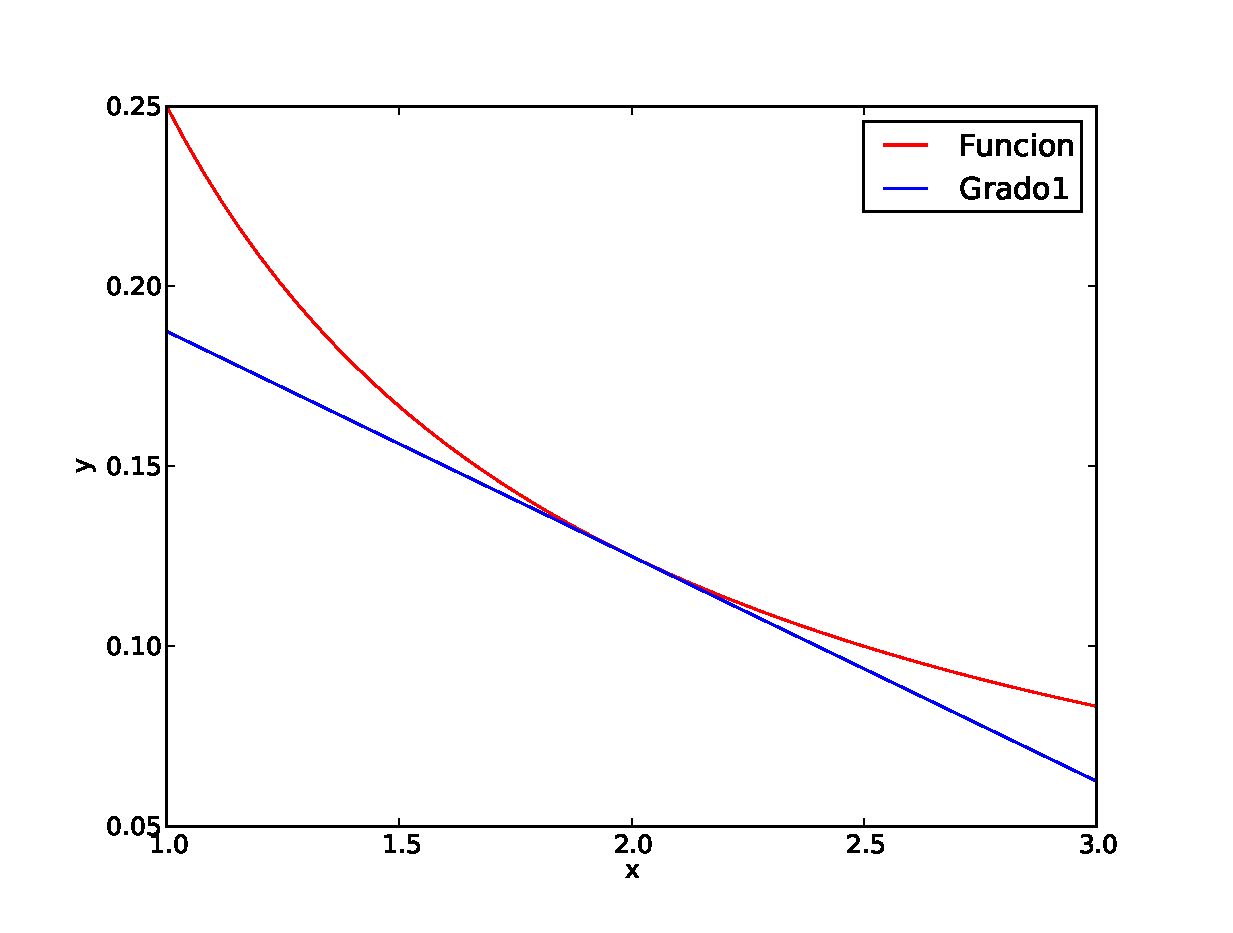
\includegraphics[scale=.6]{segunda.eps}
    \caption{Gráfica 1} 
   
  \end{center}
\end{figure}

\newpage

\begin{table}[!hbt]
\begin{center}
\begin{tabular}[c]{||l | l ||l|l||}
\hline
\hline
$x$  & $f(x)=\frac{1}{4x}$ &{\em Taylor} & Error \\
\hline
1 &0.25 & 0.21875 &12.5 \\
\hline
1.5 &0.1666667  & 0.1640625& 1.5625  \\
\hline
2 &0.125 &0.125 &  0 \\
\hline
2.5 &0.1 &0.1015625 & 1.5625  \\
\hline
3 &  0.08333 &  0.09375& 12.5  \\
\hline
\hline
\end{tabular}
\caption{La $c$ vale 2 y está interpolada en grado 2}
\end{center}
\end{table}

\begin{figure}[ht]
  \begin{center}
    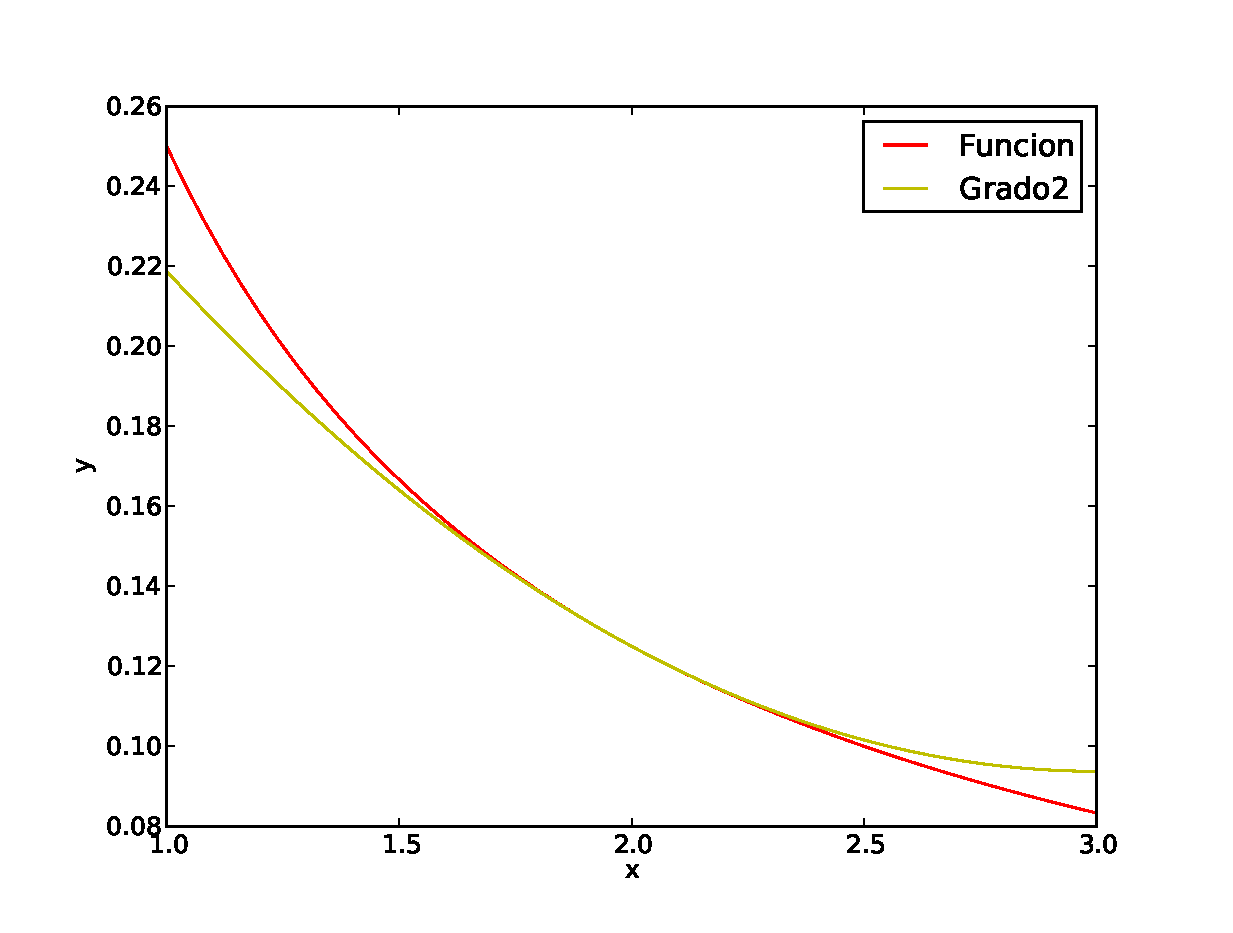
\includegraphics[scale=.6]{tercera.eps}
    \caption{Gráfica 2} 
  
  \end{center}
\end{figure}

\newpage

\begin{table}[!hbt]
\begin{center}
\begin{tabular}[c]{||l | l ||l|l||}
\hline
\hline
$x$  & $f(x)=\frac{1}{4x}$ & {\em Taylor} & Error \\
\hline
1 &0.25& 0.234375 & 6.25 \\
\hline
1.5 &0.1666667&0.166015625&  0.390625\\
\hline
2 &0.125 &0.125 &  0 \\
\hline
2.5 &0.1 &0.099609375 &  0.390625 \\
\hline
3 &  0.0.078125 &  0.234275& 6.25  \\
\hline
\hline
\end{tabular}
\caption{La $c$ vale 2 y está interpolada en grado 3}
\end{center}
\end{table}

\begin{figure}[ht]
  \begin{center}
    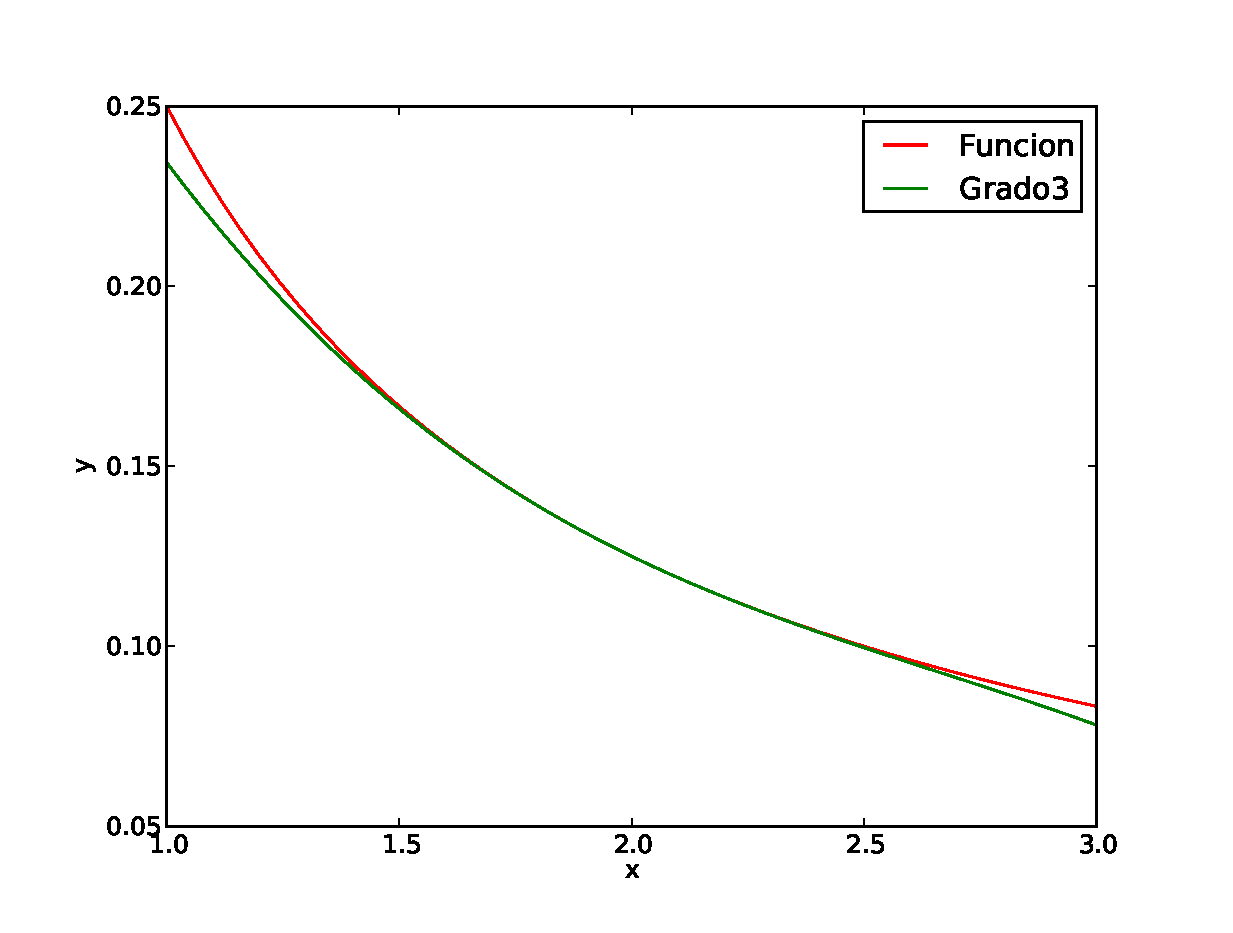
\includegraphics[scale=.6]{cuarta.eps}
    \caption{Grafica 3} 
  \end{center}
\end{figure}
\newpage
\begin{figure}[ht]
  \begin{center}
    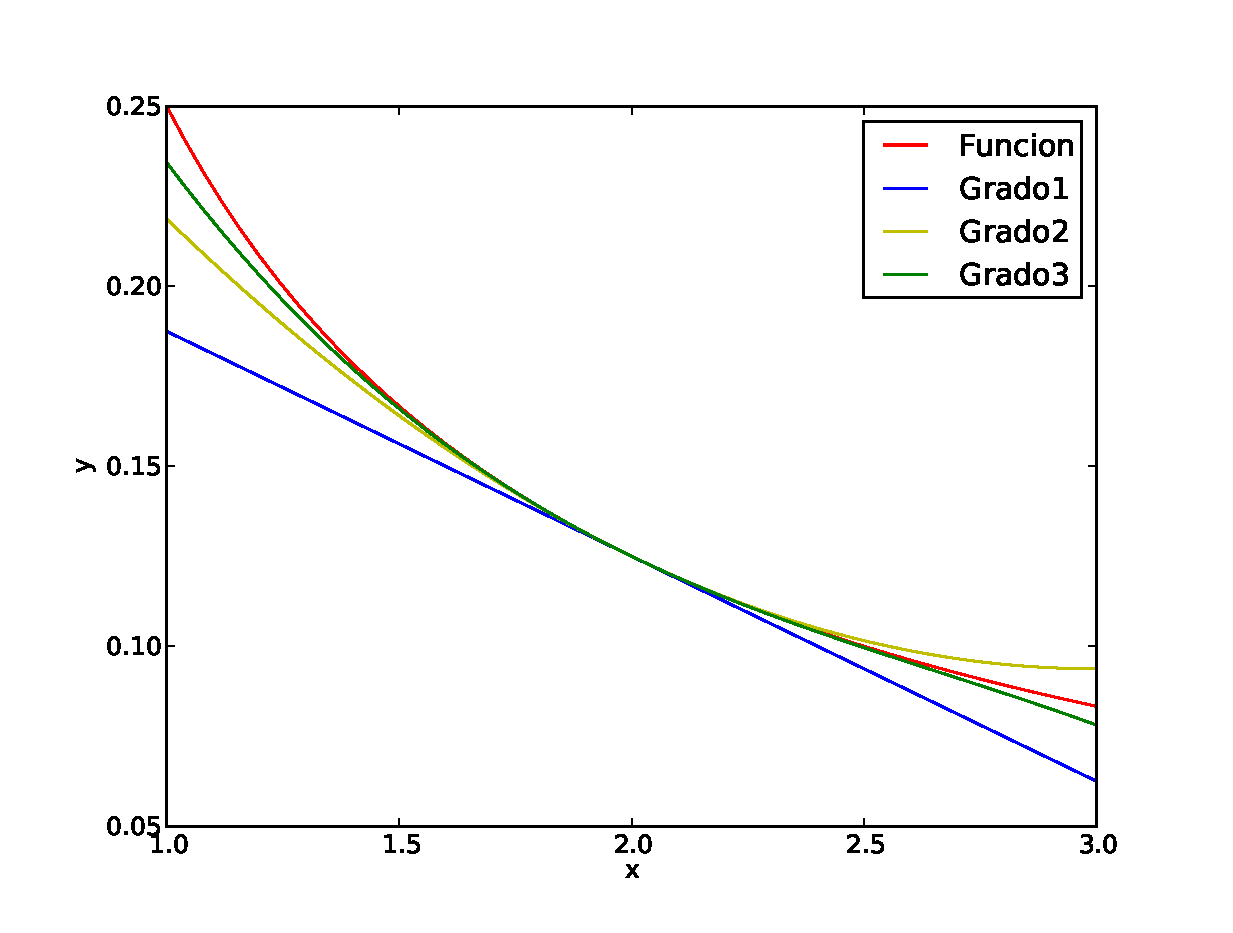
\includegraphics[scale=0.8]{sexta.eps}
    \caption{Grafica 3. Comparación de los valores anteriores} 
  \end{center}
\end{figure}


\newpage 


\subsection{Análisis de los resultados}

Observando detenidamente los resultados obtenidos mediante el expermiento realizado a cabo podemos podemos anaizar los siguientes aspectos:

En la primera tabla, donde quedan representados los datos de la primera interpolación, podemos afirmar
que el polinomio de Taylor no es tan efectivo como lo esperado pues en el punto uno y sabiendo que el 
centro es dos el error cometido por esta técnica es del 25 porciento al igual que ocurre
en el punto 3. Mientras que si observamos el punto 1.5 el rerror disminuye al acercarse al centro siendo
ahora el error de 6.25, un porcentaje algo elvado para la presicion que buscamos. Sin embargo en el punto que coincide
con el centro el error es 0 teniendo así una efectividad del cien por cien. 

Si observamos ahora la tercera tabla observamos como el error disminuye con respecto a la primera
siendo el error en el punto 1 de un 12.5 por ciento (25 porciento en la primera tabla) y en el 
punto 1.5 de tan solo 1.5625 por ciento (6.5 por ciento en la primera). Además vemos como se vuelve 
a repetir la uniformidad de la primera tabla donde el primer valor produce el mismo error que el último
mientras que el segundo error es igual al cuarto. Por último cabe destacar que en esta tabla
se vuelve a repetir la exactitud en el punto 2 que es donde el centro y el punto analizado se 
igualan. 

Por último al analizar la tercera tabla nos damos cuenta de que el error disminuye aun más, consiguiendo así 
en el punto 1 una efectividad del 93.75 por ciento al igual que en el punto 3 mientras que en el punto 1.5 y el 
2.5 se consigue una efectividad casi del cien por cien (99.609375 por ciento). Con esto también podemos afirmar
que vuelve a cumplirse el mismo modelo de repetición de la tabla uno y dos.




\newpage
\section{\textcolor{red}{Conclusión}}
Según los resultados obtenidos de las pruebas realizadas, podemos ver que a medida que el grado de la interpolación aumenta el tanto por ciento de error va disminuyendo. 
Cabe destacar que la interpolación en grado dos y en grado tres son similares.
Por otro lado, también queda decir que este tio de interpolación puede alcanzar errores muy altos, pero en este intervalo no sucede ya que es un intervalo pequeño y la función es bastante simple.

También cabe destacar, la conformidad de todos los miembros del grupo a la hora de tener que realizar el informe en {\tt Latex} ya que esto nos has proporcionado una mayor soltura con este tipo 
de paquete, uno de los objetivos principales de la asignatura para el que ha sido requerido toda esta información. Además, todo esto nos ha proporcionado conocimientos 
que nos será util para trabajos futuros como el proyecto final de grado.


Hemos de decir que a pesar de la dificultad que nos ha presentado la realización de este informe, nos encontramos  satisfechos con los resultados obtenidos. 
Esto implica que hemos conseguido simplificar la función inicial que se nos ha expuesto, objetivo principal de la interpolación de {\em Taylor}, y hallar la representación de esta nueva función.
Además, al comparar  la función interpolada con la inicial hemos verificado que este método es una  aproximación de los valores resultantes.
\newpage
\section{\textcolor{red}{Algoritmos utilizados}}
\subsection{Algoritmo Phython para analizar el polinomio de Taylor}

 Nombre: Pythonfinal.py
 
 

\underline{Descripción:}

Este programa esta compuesto por 4 funciones, las cuales nos dan un resultado final donde se puede diferenciar el valor de la interpolacion el de la función y el del 
error cometido por Tyalor.

Si comenzamos analizando el programa podemos observar que en la parte principal del programa lo primero que se pide por teclado son el punto de análisis, el grado de la interpolación
y el centro de la misma. Luego hay una primera impresión por pantalla donde se llama a dos valores y a la funcion taylor. A esta función pasamos tres parametros recogidos 
por comando (el grado, el punto y el centro). Dentro de la función Tyalor definimos una nueva variable ``sum'' y la igualamos a 0. A continuación mediante un bucle de i en 
el rango compuesto por el grado de la interpolación derivamos la función y le sumamos a la variable ``sum'' esa parte de la interpolación hasta completarla y por último retornar
su valor final a la función que luego será impresa por pantalla.

En la segunda impresión del programa es invoca a la función ``fun'' a la que solo pasamos el valor de x. Esta función es la encargada de calcular 
el valor de $f(x)=\frac{1}{4x}$ en el punto que queremos analizar.
  
Por último la tercera impresión nos mostrará por pantalla el error aproximado cometido por la función de Tyalor y esto lo hace invocando a la función ``error'' que recibe
desde la linea de comando el centro, el grado de interpolación y el punto a analizar. Dentro de esta función se llama a las dos funciones citadas anteriormente y obtiene su valor
una vez halladas calcula el valor absoluto de la diferencia entre el valor aproximado obtenido por Tyalor y el valor real de la función, esto es dividio entre el valor real
de la función y multiplicado por 100 para así calcular el tanto porciento de error. 


\begin{verbatim}
#!/usr/bin/python
import  sys
from sympy import *
from math import *

symb_c = Symbol('c')
symb_x = Symbol('x')
func = 1/(4*symb_c)



def fac(i):
    if i == 0:
	return 1
    else:
	return i * fac(i-1)
	
def taylor(c, x, n):
  
  sum=0
  for i in range(n):
    derivada= diff(func, symb_c, i)

    sum+=((eval(str(derivada)))/((fac(i)))*((x-c)**(i)))
    
  return sum
  
def fun(x):
  
  func = 1/(4*symb_x)
  sum2= eval(str(func))
  return sum2
  
  
def error(c, x, n):
  error=(abs((taylor(c, x, n))-(fun(x))))/(fun(x)) * 100
  return error
    
if __name__ == '__main__':
  n=int(sys.argv[1])
  x=float(sys.argv[2])
  c=float(sys.argv[3])
    
  print "El resultado de evaluar el ploinomio de Taylor de grado
  
  {0} en el punto {1} es {2}".format(n, x, taylor(c, x, n))
  print "El resultado de evaluar la funcion en el punto {0} es: 
  
  {1}".format(c,fun(x))
  print "El error cometido por el polinomio de Taylor es de: 
  
  {0}".format(error(c, x, n))
\end{verbatim}
\subsection{Algoritmo para las gráficas}


\underline{Descripción:}

El algoritmo propuesto a continuación es el encargado de proporcionarnos una gŕafica en la que quedan representadas las tres funciones de Tyalor y la función propuesta
para analizar. En la primera parte del programa se definen las cuatro funciones que se van a representar. Luego se define el intervalo en el que actuará la variable y 
los puntos que queremos representar. Justo después es necesario reservar el mismo espacio puesto en la variable par las imagenes de la función, y a continuación mediante un
bucle se igualan las imagenes a las variables en todo el rango propuesto. Este proceso se repite tres veces mas para las tres funciones de Tyalor. Por último se determinan
las formas y colores de la representación gráfica de cada función y se añade una leyenda. 

Cabe destacar que este algoritmo nos ha servido para representar todas las gráficas adjuntadas en el documento pues simplemente nos ha hecho falta redefinir las funciones
y cambiar algún parámetro. 





\begin{verbatim}

from matplotlib.pylab import *
# Mostrar mas de una representacion en el mismo lienzo 

diagrama1 = figure(1)

# la figura tendra 2 filas y 1 columna y se quiere trazar en la primera


def g(x):
  
  return 1/(4*x)
  
def f(x):
#En este caso c vale 2
  
  return (0.125-(0.0625)*(x-2))
  
def t(x):
#En este caso c vale 2
  
  return ((0.125-(0.0625)*(x-2))+(0.03125)*(x-2)**2)
  
def p(x):
#En este caso c vale 2
 
  return ((0.125-(0.0625)*(x-2))+(0.03125)*(x-2)**2-(0.015625)*(x-2)**3)
  

x = linspace(1, 3, 51)  # 51 puntos entre 0 y 3
y = zeros(len(x))       # reserva memoria para y con elementos flotantes
for i in xrange(len(x)):
  y[i] = g(x[i])



x = linspace(1, 3, 51)  # 51 puntos entre 0 y 3
h = zeros(len(x))       # reserva memoria para y con elementos flotantes
for i in xrange(len(x)):
  h[i] = f(x[i])
  
  
x = linspace(1, 3, 51)  # 51 puntos entre 0 y 3
z = zeros(len(x))       # reserva memoria para y con elementos flotantes
for i in xrange(len(x)):
  z[i] = t(x[i])
  
x = linspace(1, 3, 51)  # 51 puntos entre 0 y 3
w = zeros(len(x))       # reserva memoria para y con elementos flotantes
for i in xrange(len(x)):
  w[i] = p(x[i])
  

plot0= plot(x,y, 'r')
plot1= plot(x,h,'b')
plot2= plot(x,z,'y')
plot3= plot(x,w,'g')

xlabel('x')
ylabel('y')

legend(['Funcion', 'Grado1', 'Grado2', 'Grado3'])

show()

\end{verbatim}




\newpage
\section{\textcolor{red}{Bibliografía}}
La información requerida para la realización de este informe ha sido extraída de las siguientes fuentes:
\begin{itemize}
\item {$disi.unal.edu.co/~lctorres/MetNum/MeNuI03.pdf$}
\item {$www.ugr.es/~mpasadas/ftp/Inter2.pdf$}
\item {$cse.web.cs.illinois.edu/iem/interpolation/taylor/$}
\item {$http://www.fceia.unr.edu.ar/lcc/cdrom/Instalaciones/LaTex/latex.html$}
\item {$http://es.wikipedia.org/wiki/Interpolaci$}
\item {$youtube.com$}
\end {itemize}

\bigskip
\end{document}